\documentclass[tikz,border=4pt]{standalone}
\usepackage[T1]{fontenc}
\usepackage[utf8]{inputenc}
\usepackage{FiraSans}
\usepackage{amsmath}
\usetikzlibrary{arrows.meta,positioning,calc,fit}
\definecolor{ceBlue}{RGB}{42,96,153}
\definecolor{ceTeal}{RGB}{36,135,118}
\definecolor{ceGold}{RGB}{220,160,52}
\definecolor{ceRed}{RGB}{188,74,60}
\definecolor{ceInk}{RGB}{42,42,42}
\definecolor{ceGray}{RGB}{238,240,242}
\begin{document}
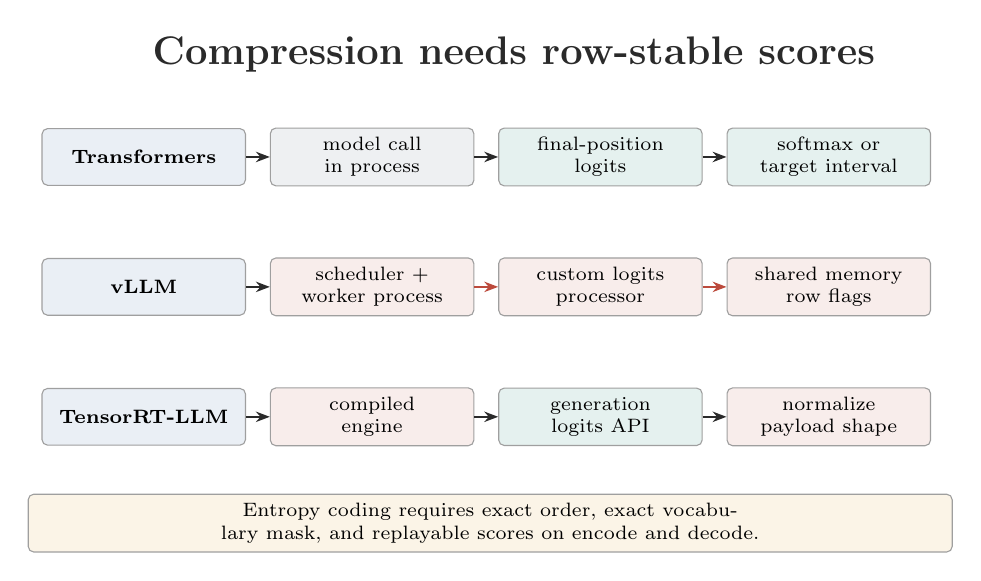
\begin{tikzpicture}[
  x=1cm,y=1cm,
  font=\sffamily,
  box/.style={draw=ceInk!45, rounded corners=2pt, minimum height=0.72cm, text width=2.35cm, align=center, font=\scriptsize, fill=white},
  engine/.style={box, fill=ceBlue!10, font=\scriptsize\bfseries},
  host/.style={box, fill=ceGray},
  hard/.style={box, fill=ceRed!10},
  good/.style={box, fill=ceTeal!12},
  arr/.style={-{Stealth[length=5pt]}, thick, ceInk},
  warn/.style={-{Stealth[length=5pt]}, thick, ceRed},
]
  \node[font=\Large\bfseries, ceInk] at (6.4,6.3) {Compression needs row-stable scores};

  \node[engine] (tr) at (1.7,5.0) {Transformers};
  \node[host] (trh) at (4.6,5.0) {model call\\in process};
  \node[good] (trl) at (7.5,5.0) {final-position\\logits};
  \node[good] (trc) at (10.4,5.0) {softmax or\\target interval};
  \draw[arr] (tr) -- (trh);
  \draw[arr] (trh) -- (trl);
  \draw[arr] (trl) -- (trc);

  \node[engine] (vl) at (1.7,3.35) {vLLM};
  \node[hard] (vls) at (4.6,3.35) {scheduler +\\worker process};
  \node[hard] (vlp) at (7.5,3.35) {custom logits\\processor};
  \node[hard] (vlm) at (10.4,3.35) {shared memory\\row flags};
  \draw[arr] (vl) -- (vls);
  \draw[warn] (vls) -- (vlp);
  \draw[warn] (vlp) -- (vlm);

  \node[engine] (tt) at (1.7,1.7) {TensorRT-LLM};
  \node[hard] (tte) at (4.6,1.7) {compiled\\engine};
  \node[good] (ttg) at (7.5,1.7) {generation\\logits API};
  \node[hard] (ttn) at (10.4,1.7) {normalize\\payload shape};
  \draw[arr] (tt) -- (tte);
  \draw[arr] (tte) -- (ttg);
  \draw[arr] (ttg) -- (ttn);

  \node[box, fill=ceGold!12, text width=11.5cm, minimum height=0.7cm] at (6.1,0.35)
    {Entropy coding requires exact order, exact vocabulary mask, and replayable scores on encode and decode.};
\end{tikzpicture}
\end{document}
